\subsection{Results}\label{subsec:results}
AE latent blending vs. VAE latent blending vs. linear interpolation (take a motion add gaps, fill gaps, record MSE)

insert some examples here (image sequences) of good results and bad results

\subsubsection{Autoencoder}\label{subsubsec:autoencoder}
The autoencoder has been trained to encode a pose. The training then optimizes the MSE loss between the original pose and the autoencoded pose. While training we record the loss for the training dataset and the test dataset at the end of each epoch. A graph of the test and training loss over the epochs can be seen in \autoref{fig:ae-loss}. There is a large gap between the training and test loss. This is because there are poses in the test dataset that are very far away from the train dataset, \autoref{fig:test-turning} shows an example of such a motion in the test dataset. Having a larger dataset would help alleviate this. Since both the training and test loss decrease monotonically over time there is no indication of overfitting.

\begin{figure}[h]
\centering
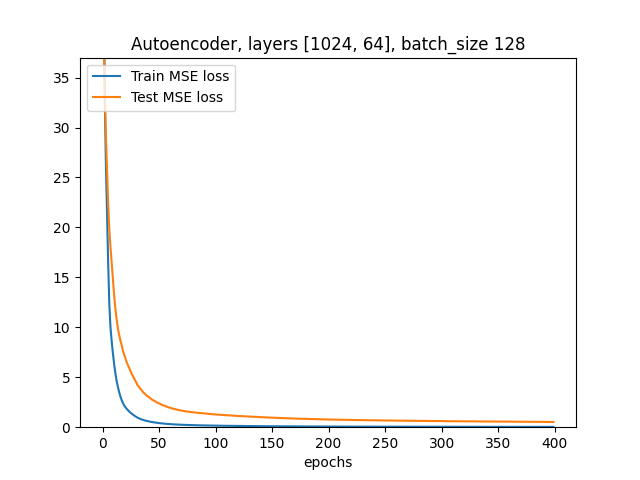
\includegraphics[width=0.5\textwidth]{img/simple_1024-64_batch-128_losses}
\caption{Loss over epochs for the autoencoder. The reconstruction\_loss is the MSE loss and the kld\_loss is not applicable for this model.}
\label{fig:ae-loss}
\end{figure}

\begin{figure}[h]
\centering
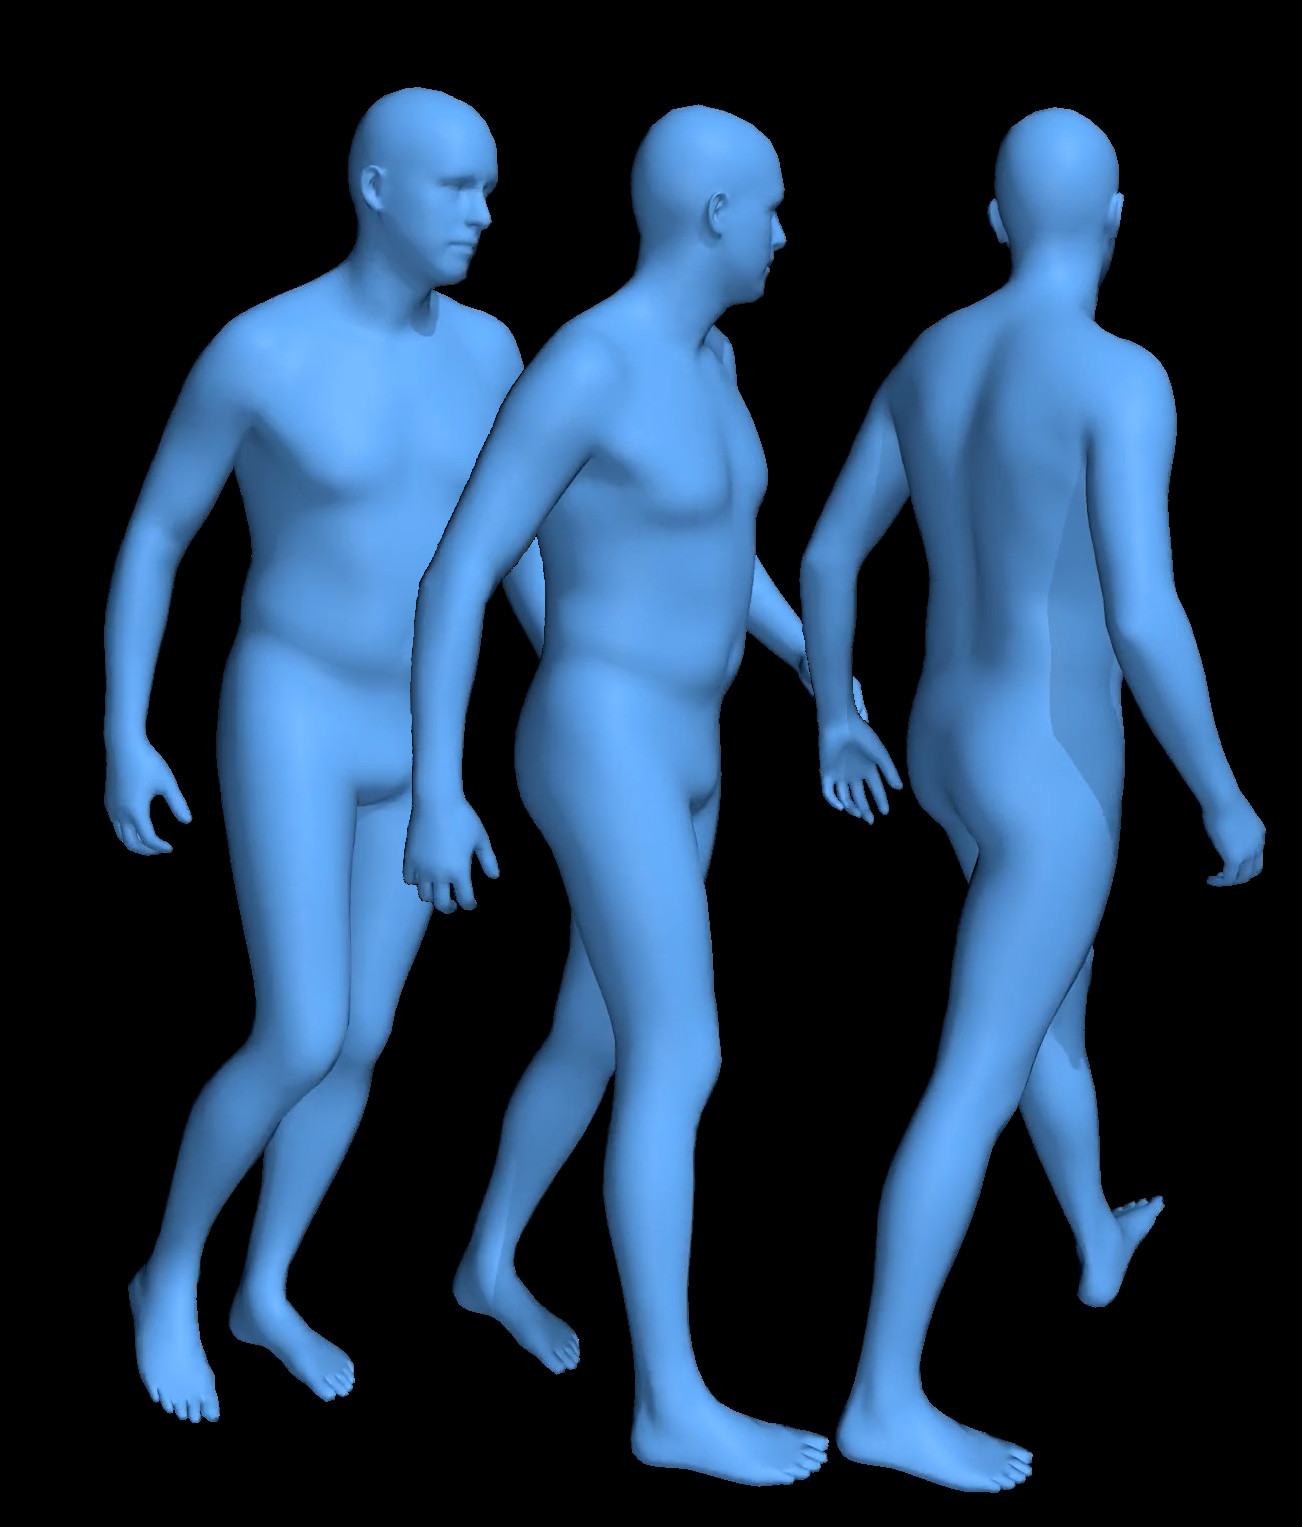
\includegraphics[width=0.3\textwidth]{img/46_01_turning}
\caption{Subject 46, trial 1 from the CMU dataset. The motion depicts turning around, as opposed to simply walking straight ahead.}
\label{fig:test-turning}
\end{figure}
% TODO: Examples below, both whole anim and inpaint


\subsubsection{Variational autoencoder}\label{subsubsec:vae}
\begin{figure}[h]
\centering
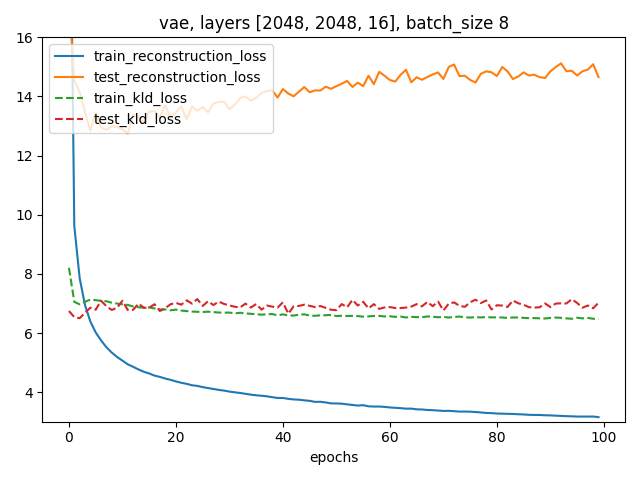
\includegraphics[width=0.5\textwidth]{img/vae_2048-2048-16_batch-8_losses}
\caption{TODO}
\label{fig:vae-loss}
\end{figure}


\subsection{Further research}\label{subsec:further-research}
clustered-specialists-paper~\cite{won2020scalable}

something about motion prediction maybe (a way to utilize forwards/backwards info)

closer comparison with existing motion prediction models

using vq-vae

using the full amass data training
